\paragraph{MDPs: Bonus level!}
\begin{center}
\centering
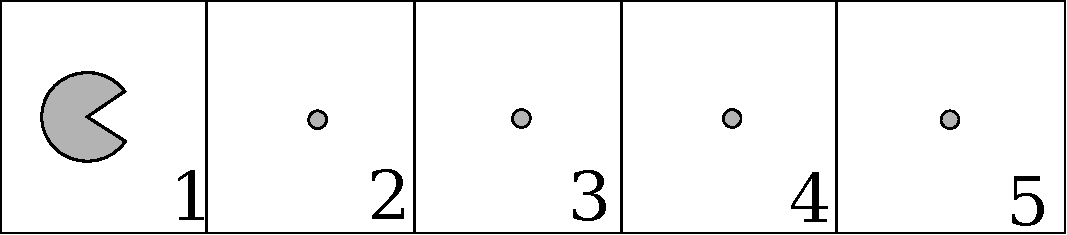
\includegraphics[height=2.1cm]{figures/drawing2.pdf}
\vspace{1mm}
\end{center}

Pacman is in a bonus level! With no ghosts around, he can eat as many dots as he wants. He is in the 5 $\times$ 1 grid shown. The cells are numbered from left to right as $1,\ldots, 5$. In cells 1 through 4, the actions available to him are to move \emph{Right} (R) or to \emph{Fly} (F) out of the bonus level. The action \emph{Right} deterministically lands Pacman in the cell to the right (and he eats the dot there), while the \emph{Fly} action deterministically lands him in a terminal state and ends the game. From cell 5, \emph{Fly} is the only action.  Eating a dot gives a reward of $10$, while flying out gives a reward of $20$. Pacman starts in the leftmost cell (cell 1).

We write this as an MDP where the state is the cell that Pacman is in. The discount is $\gamma$.

Consider the following 3 policies:
\begin{align*}
\pi_0(s) &= F \textrm{ for all } s \\
\pi_1(s) &= R \textrm{ if }s \leq 3,\ F \textrm{ otherwise }\\
\pi_2(s) &= R \textrm{ if }s \leq 4,\ F \textrm{ otherwise }
\end{align*}

\begin{enumerate}


\item Assume $\gamma=1.0$. What is:
\vspace{10mm}
\begin{enumerate}
\item $V^{\pi_0}(1)$? \\
{\color{red}20}
\item $V^{\pi_1}(1)$? \\
{\color{red}50}
\item $V^{\pi_2}(1)$? \\
{\color{red}60}
\item $V^*(1)$? \\
{\color{red}60}
\end{enumerate}
\vfill

\end{enumerate}